\documentclass[1p]{elsarticle_modified}
%\bibliographystyle{elsarticle-num}

%\usepackage[colorlinks]{hyperref}
%\usepackage{abbrmath_seonhwa} %\Abb, \Ascr, \Acal ,\Abf, \Afrak
\usepackage{amsfonts}
\usepackage{amssymb}
\usepackage{amsmath}
\usepackage{amsthm}
\usepackage{scalefnt}
\usepackage{amsbsy}
\usepackage{kotex}
\usepackage{caption}
\usepackage{subfig}
\usepackage{color}
\usepackage{graphicx}
\usepackage{xcolor} %% white, black, red, green, blue, cyan, magenta, yellow
\usepackage{float}
\usepackage{setspace}
\usepackage{hyperref}

\usepackage{tikz}
\usetikzlibrary{arrows}

\usepackage{multirow}
\usepackage{array} % fixed length table
\usepackage{hhline}

%%%%%%%%%%%%%%%%%%%%%
\makeatletter
\renewcommand*\env@matrix[1][\arraystretch]{%
	\edef\arraystretch{#1}%
	\hskip -\arraycolsep
	\let\@ifnextchar\new@ifnextchar
	\array{*\c@MaxMatrixCols c}}
\makeatother %https://tex.stackexchange.com/questions/14071/how-can-i-increase-the-line-spacing-in-a-matrix
%%%%%%%%%%%%%%%

\usepackage[normalem]{ulem}

\newcommand{\msout}[1]{\ifmmode\text{\sout{\ensuremath{#1}}}\else\sout{#1}\fi}
%SOURCE: \msout is \stkout macro in https://tex.stackexchange.com/questions/20609/strikeout-in-math-mode

\newcommand{\cancel}[1]{
	\ifmmode
	{\color{red}\msout{#1}}
	\else
	{\color{red}\sout{#1}}
	\fi
}

\newcommand{\add}[1]{
	{\color{blue}\uwave{#1}}
}

\newcommand{\replace}[2]{
	\ifmmode
	{\color{red}\msout{#1}}{\color{blue}\uwave{#2}}
	\else
	{\color{red}\sout{#1}}{\color{blue}\uwave{#2}}
	\fi
}

\newcommand{\Sol}{\mathcal{S}} %segment
\newcommand{\D}{D} %diagram
\newcommand{\A}{\mathcal{A}} %arc


%%%%%%%%%%%%%%%%%%%%%%%%%%%%%5 test

\def\sl{\operatorname{\textup{SL}}(2,\Cbb)}
\def\psl{\operatorname{\textup{PSL}}(2,\Cbb)}
\def\quan{\mkern 1mu \triangleright \mkern 1mu}

\theoremstyle{definition}
\newtheorem{thm}{Theorem}[section]
\newtheorem{prop}[thm]{Proposition}
\newtheorem{lem}[thm]{Lemma}
\newtheorem{ques}[thm]{Question}
\newtheorem{cor}[thm]{Corollary}
\newtheorem{defn}[thm]{Definition}
\newtheorem{exam}[thm]{Example}
\newtheorem{rmk}[thm]{Remark}
\newtheorem{alg}[thm]{Algorithm}

\newcommand{\I}{\sqrt{-1}}
\begin{document}

%\begin{frontmatter}
%
%\title{Boundary parabolic representations of knots up to 8 crossings}
%
%%% Group authors per affiliation:
%\author{Yunhi Cho} 
%\address{Department of Mathematics, University of Seoul, Seoul, Korea}
%\ead{yhcho@uos.ac.kr}
%
%
%\author{Seonhwa Kim} %\fnref{s_kim}}
%\address{Center for Geometry and Physics, Institute for Basic Science, Pohang, 37673, Korea}
%\ead{ryeona17@ibs.re.kr}
%
%\author{Hyuk Kim}
%\address{Department of Mathematical Sciences, Seoul National University, Seoul 08826, Korea}
%\ead{hyukkim@snu.ac.kr}
%
%\author{Seokbeom Yoon}
%\address{Department of Mathematical Sciences, Seoul National University, Seoul, 08826,  Korea}
%\ead{sbyoon15@snu.ac.kr}
%
%\begin{abstract}
%We find all boundary parabolic representation of knots up to 8 crossings.
%
%\end{abstract}
%\begin{keyword}
%    \MSC[2010] 57M25 
%\end{keyword}
%
%\end{frontmatter}

%\linenumbers
%\tableofcontents
%
\newcommand\colored[1]{\textcolor{white}{\rule[-0.35ex]{0.8em}{1.4ex}}\kern-0.8em\color{red} #1}%
%\newcommand\colored[1]{\textcolor{white}{ #1}\kern-2.17ex	\textcolor{white}{ #1}\kern-1.81ex	\textcolor{white}{ #1}\kern-2.15ex\color{red}#1	}

{\Large $\underline{12a_{0740}~(K12a_{0740})}$}

\setlength{\tabcolsep}{10pt}
\renewcommand{\arraystretch}{1.6}
\vspace{1cm}\begin{tabular}{m{100pt}>{\centering\arraybackslash}m{274pt}}
\multirow{5}{120pt}{
	\centering
	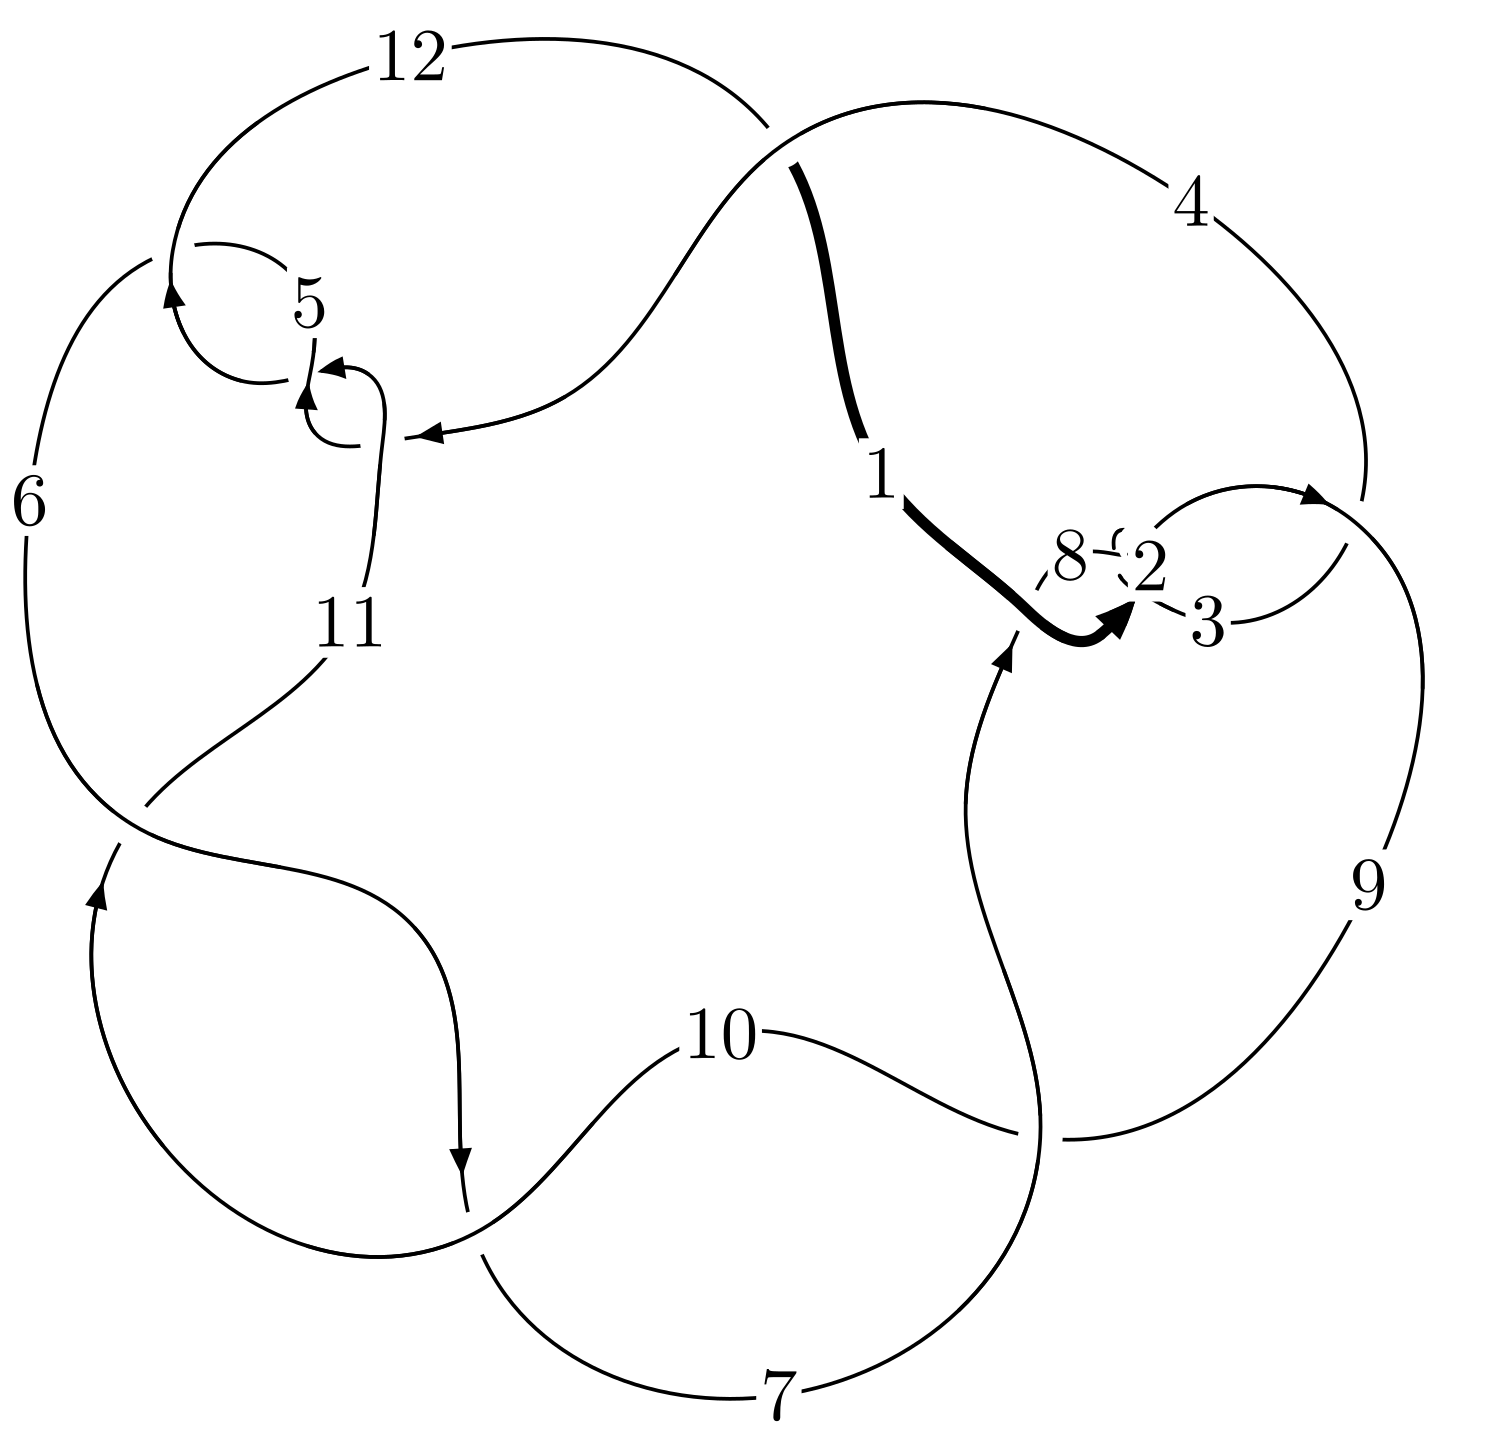
\includegraphics[width=112pt]{../../../GIT/diagram.site/Diagrams/png/1541_12a_0740.png}\\
\ \ \ A knot diagram\footnotemark}&
\allowdisplaybreaks
\textbf{Linearized knot diagam} \\
\cline{2-2}
 &
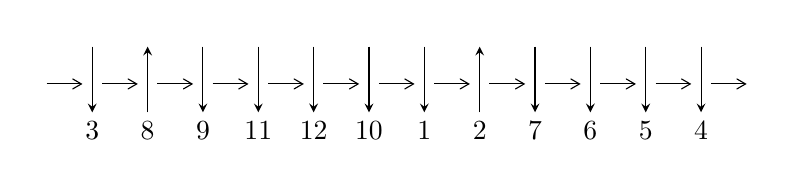
\begin{tikzpicture}[x=20pt, y=17pt]
	% nodes
	\node (C0) at (0, 0) {};
	\node (C1) at (1, 0) {};
	\node (C1U) at (1, +1) {};
	\node (C1D) at (1, -1) {3};

	\node (C2) at (2, 0) {};
	\node (C2U) at (2, +1) {};
	\node (C2D) at (2, -1) {8};

	\node (C3) at (3, 0) {};
	\node (C3U) at (3, +1) {};
	\node (C3D) at (3, -1) {9};

	\node (C4) at (4, 0) {};
	\node (C4U) at (4, +1) {};
	\node (C4D) at (4, -1) {11};

	\node (C5) at (5, 0) {};
	\node (C5U) at (5, +1) {};
	\node (C5D) at (5, -1) {12};

	\node (C6) at (6, 0) {};
	\node (C6U) at (6, +1) {};
	\node (C6D) at (6, -1) {10};

	\node (C7) at (7, 0) {};
	\node (C7U) at (7, +1) {};
	\node (C7D) at (7, -1) {1};

	\node (C8) at (8, 0) {};
	\node (C8U) at (8, +1) {};
	\node (C8D) at (8, -1) {2};

	\node (C9) at (9, 0) {};
	\node (C9U) at (9, +1) {};
	\node (C9D) at (9, -1) {7};

	\node (C10) at (10, 0) {};
	\node (C10U) at (10, +1) {};
	\node (C10D) at (10, -1) {6};

	\node (C11) at (11, 0) {};
	\node (C11U) at (11, +1) {};
	\node (C11D) at (11, -1) {5};

	\node (C12) at (12, 0) {};
	\node (C12U) at (12, +1) {};
	\node (C12D) at (12, -1) {4};
	\node (C13) at (13, 0) {};

	% arrows
	\draw[->,>={angle 60}]
	(C0) edge (C1) (C1) edge (C2) (C2) edge (C3) (C3) edge (C4) (C4) edge (C5) (C5) edge (C6) (C6) edge (C7) (C7) edge (C8) (C8) edge (C9) (C9) edge (C10) (C10) edge (C11) (C11) edge (C12) (C12) edge (C13) ;	\draw[->,>=stealth]
	(C1U) edge (C1D) (C2D) edge (C2U) (C3U) edge (C3D) (C4U) edge (C4D) (C5U) edge (C5D) (C6U) edge (C6D) (C7U) edge (C7D) (C8D) edge (C8U) (C9U) edge (C9D) (C10U) edge (C10D) (C11U) edge (C11D) (C12U) edge (C12D) ;
	\end{tikzpicture} \\
\hhline{~~} \\& 
\textbf{Solving Sequence} \\ \cline{2-2} 
 &
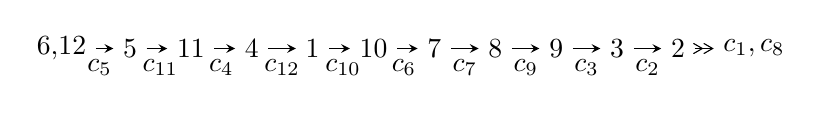
\begin{tikzpicture}[x=22pt, y=7pt]
	% node
	\node (A0) at (-1/8, 0) {6,12};
	\node (A1) at (1, 0) {5};
	\node (A2) at (2, 0) {11};
	\node (A3) at (3, 0) {4};
	\node (A4) at (4, 0) {1};
	\node (A5) at (5, 0) {10};
	\node (A6) at (6, 0) {7};
	\node (A7) at (7, 0) {8};
	\node (A8) at (8, 0) {9};
	\node (A9) at (9, 0) {3};
	\node (A10) at (10, 0) {2};
	\node (C1) at (1/2, -1) {$c_{5}$};
	\node (C2) at (3/2, -1) {$c_{11}$};
	\node (C3) at (5/2, -1) {$c_{4}$};
	\node (C4) at (7/2, -1) {$c_{12}$};
	\node (C5) at (9/2, -1) {$c_{10}$};
	\node (C6) at (11/2, -1) {$c_{6}$};
	\node (C7) at (13/2, -1) {$c_{7}$};
	\node (C8) at (15/2, -1) {$c_{9}$};
	\node (C9) at (17/2, -1) {$c_{3}$};
	\node (C10) at (19/2, -1) {$c_{2}$};
	\node (A11) at (45/4, 0) {$c_{1},c_{8}$};

	% edge
	\draw[->,>=stealth]	
	(A0) edge (A1) (A1) edge (A2) (A2) edge (A3) (A3) edge (A4) (A4) edge (A5) (A5) edge (A6) (A6) edge (A7) (A7) edge (A8) (A8) edge (A9) (A9) edge (A10) ;
	\draw[->>,>={angle 60}]	
	(A10) edge (A11);
\end{tikzpicture} \\ 

\end{tabular} \\

\footnotetext{
The image of knot diagram is generated by the software ``\textbf{Draw programme}" developed by Andrew Bartholomew(\url{http://www.layer8.co.uk/maths/draw/index.htm\#Running-draw}), where we modified some parts for our purpose(\url{https://github.com/CATsTAILs/LinksPainter}).
}\phantom \\ \newline 
\centering \textbf{Ideals for irreducible components\footnotemark of $X_{\text{par}}$} 
 
\begin{align*}
I^u_{1}&=\langle 
u^{56}+u^{55}+\cdots-2 u-1\rangle \\
\\
\end{align*}
\raggedright * 1 irreducible components of $\dim_{\mathbb{C}}=0$, with total 56 representations.\\
\footnotetext{All coefficients of polynomials are rational numbers. But the coefficients are sometimes approximated in decimal forms when there is not enough margin.}
\newpage
\renewcommand{\arraystretch}{1}
\centering \section*{I. $I^u_{1}= \langle u^{56}+u^{55}+\cdots-2 u-1 \rangle$}
\flushleft \textbf{(i) Arc colorings}\\
\begin{tabular}{m{7pt} m{180pt} m{7pt} m{180pt} }
\flushright $a_{6}=$&$\begin{pmatrix}1\\0\end{pmatrix}$ \\
\flushright $a_{12}=$&$\begin{pmatrix}0\\u\end{pmatrix}$ \\
\flushright $a_{5}=$&$\begin{pmatrix}1\\- u^2\end{pmatrix}$ \\
\flushright $a_{11}=$&$\begin{pmatrix}u\\- u^3+u\end{pmatrix}$ \\
\flushright $a_{4}=$&$\begin{pmatrix}- u^2+1\\u^4-2 u^2\end{pmatrix}$ \\
\flushright $a_{1}=$&$\begin{pmatrix}- u^5+2 u^3- u\\u^7-3 u^5+2 u^3+u\end{pmatrix}$ \\
\flushright $a_{10}=$&$\begin{pmatrix}- u^3+2 u\\- u^3+u\end{pmatrix}$ \\
\flushright $a_{7}=$&$\begin{pmatrix}u^6-3 u^4+2 u^2+1\\u^6-2 u^4+u^2\end{pmatrix}$ \\
\flushright $a_{8}=$&$\begin{pmatrix}- u^{18}+7 u^{16}-20 u^{14}+27 u^{12}-11 u^{10}-13 u^8+16 u^6-6 u^4+u^2+1\\u^{20}-8 u^{18}+26 u^{16}-40 u^{14}+19 u^{12}+24 u^{10}-30 u^8+2 u^6+5 u^4+2 u^2\end{pmatrix}$ \\
\flushright $a_{9}=$&$\begin{pmatrix}- u^9+4 u^7-5 u^5+3 u\\- u^9+3 u^7-3 u^5+u\end{pmatrix}$ \\
\flushright $a_{3}=$&$\begin{pmatrix}u^{22}-9 u^{20}+\cdots-4 u^2+1\\u^{22}-8 u^{20}+\cdots-4 u^4-3 u^2\end{pmatrix}$ \\
\flushright $a_{2}=$&$\begin{pmatrix}- u^{51}+20 u^{49}+\cdots+11 u^3-2 u\\- u^{51}+19 u^{49}+\cdots+5 u^3+u\end{pmatrix}$\\&\end{tabular}
\flushleft \textbf{(ii) Obstruction class $= -1$}\\~\\
\flushleft \textbf{(iii) Cusp Shapes $= -4 u^{53}+80 u^{51}+\cdots-12 u-10$}\\~\\
\newpage\renewcommand{\arraystretch}{1}
\flushleft \textbf{(iv) u-Polynomials at the component}\newline \\
\begin{tabular}{m{50pt}|m{274pt}}
Crossings & \hspace{64pt}u-Polynomials at each crossing \\
\hline $$\begin{aligned}c_{1}\end{aligned}$$&$\begin{aligned}
&u^{56}+29 u^{55}+\cdots-10 u^2+1
\end{aligned}$\\
\hline $$\begin{aligned}c_{2},c_{8}\end{aligned}$$&$\begin{aligned}
&u^{56}- u^{55}+\cdots-2 u^3-1
\end{aligned}$\\
\hline $$\begin{aligned}c_{3},c_{7}\end{aligned}$$&$\begin{aligned}
&u^{56}+u^{55}+\cdots+80 u-53
\end{aligned}$\\
\hline $$\begin{aligned}c_{4},c_{5},c_{11}\end{aligned}$$&$\begin{aligned}
&u^{56}+u^{55}+\cdots-2 u-1
\end{aligned}$\\
\hline $$\begin{aligned}c_{6},c_{9},c_{10}\\c_{12}\end{aligned}$$&$\begin{aligned}
&u^{56}-3 u^{55}+\cdots-4 u+1
\end{aligned}$\\
\hline
\end{tabular}\\~\\
\newpage\renewcommand{\arraystretch}{1}
\flushleft \textbf{(v) Riley Polynomials at the component}\newline \\
\begin{tabular}{m{50pt}|m{274pt}}
Crossings & \hspace{64pt}Riley Polynomials at each crossing \\
\hline $$\begin{aligned}c_{1}\end{aligned}$$&$\begin{aligned}
&y^{56}-3 y^{55}+\cdots-20 y+1
\end{aligned}$\\
\hline $$\begin{aligned}c_{2},c_{8}\end{aligned}$$&$\begin{aligned}
&y^{56}+29 y^{55}+\cdots-10 y^2+1
\end{aligned}$\\
\hline $$\begin{aligned}c_{3},c_{7}\end{aligned}$$&$\begin{aligned}
&y^{56}-35 y^{55}+\cdots-20180 y+2809
\end{aligned}$\\
\hline $$\begin{aligned}c_{4},c_{5},c_{11}\end{aligned}$$&$\begin{aligned}
&y^{56}-43 y^{55}+\cdots+30 y^2+1
\end{aligned}$\\
\hline $$\begin{aligned}c_{6},c_{9},c_{10}\\c_{12}\end{aligned}$$&$\begin{aligned}
&y^{56}+65 y^{55}+\cdots+20 y+1
\end{aligned}$\\
\hline
\end{tabular}\\~\\
\newpage\flushleft \textbf{(vi) Complex Volumes and Cusp Shapes}
$$\begin{array}{c|c|c}  
\text{Solutions to }I^u_{1}& \I (\text{vol} + \sqrt{-1}CS) & \text{Cusp shape}\\
 \hline 
\begin{aligned}
u &= \phantom{-}0.966138 + 0.146675 I\end{aligned}
 & -4.03618 + 3.76547 I & -9.86305 - 3.31528 I \\ \hline\begin{aligned}
u &= \phantom{-}0.966138 - 0.146675 I\end{aligned}
 & -4.03618 - 3.76547 I & -9.86305 + 3.31528 I \\ \hline\begin{aligned}
u &= -0.005719 + 0.906711 I\end{aligned}
 & \phantom{-}11.65310 + 2.42579 I & -0.94991 - 3.21386 I \\ \hline\begin{aligned}
u &= -0.005719 - 0.906711 I\end{aligned}
 & \phantom{-}11.65310 - 2.42579 I & -0.94991 + 3.21386 I \\ \hline\begin{aligned}
u &= \phantom{-}0.036344 + 0.901122 I\end{aligned}
 & \phantom{-}6.27142 - 9.00482 I & -5.29022 + 5.83508 I \\ \hline\begin{aligned}
u &= \phantom{-}0.036344 - 0.901122 I\end{aligned}
 & \phantom{-}6.27142 + 9.00482 I & -5.29022 - 5.83508 I \\ \hline\begin{aligned}
u &= -1.090050 + 0.140449 I\end{aligned}
 & -1.55041 + 0.38680 I & -5.72495 + 0. I\phantom{ +0.000000I} \\ \hline\begin{aligned}
u &= -1.090050 - 0.140449 I\end{aligned}
 & -1.55041 - 0.38680 I & -5.72495 + 0. I\phantom{ +0.000000I} \\ \hline\begin{aligned}
u &= -0.028384 + 0.898900 I\end{aligned}
 & \phantom{-}8.99836 + 4.05002 I & -2.11311 - 2.32433 I \\ \hline\begin{aligned}
u &= -0.028384 - 0.898900 I\end{aligned}
 & \phantom{-}8.99836 - 4.05002 I & -2.11311 + 2.32433 I \\ \hline\begin{aligned}
u &= \phantom{-}0.028330 + 0.883702 I\end{aligned}
 & \phantom{-}4.64419 - 0.64348 I & -7.26111 - 0.24240 I \\ \hline\begin{aligned}
u &= \phantom{-}0.028330 - 0.883702 I\end{aligned}
 & \phantom{-}4.64419 + 0.64348 I & -7.26111 + 0.24240 I \\ \hline\begin{aligned}
u &= -1.167310 + 0.233432 I\end{aligned}
 & -0.432854 + 1.119920 I & \phantom{-0.000000 } 0 \\ \hline\begin{aligned}
u &= -1.167310 - 0.233432 I\end{aligned}
 & -0.432854 - 1.119920 I & \phantom{-0.000000 } 0 \\ \hline\begin{aligned}
u &= \phantom{-}1.244770 + 0.102397 I\end{aligned}
 & -4.72176 - 2.16923 I & \phantom{-0.000000 } 0 \\ \hline\begin{aligned}
u &= \phantom{-}1.244770 - 0.102397 I\end{aligned}
 & -4.72176 + 2.16923 I & \phantom{-0.000000 } 0 \\ \hline\begin{aligned}
u &= \phantom{-}1.225110 + 0.251359 I\end{aligned}
 & -0.95561 - 5.19909 I & \phantom{-0.000000 } 0 \\ \hline\begin{aligned}
u &= \phantom{-}1.225110 - 0.251359 I\end{aligned}
 & -0.95561 + 5.19909 I & \phantom{-0.000000 } 0 \\ \hline\begin{aligned}
u &= \phantom{-}1.30697\phantom{ +0.000000I}\end{aligned}
 & -6.22222\phantom{ +0.000000I} & \phantom{-0.000000 } 0 \\ \hline\begin{aligned}
u &= \phantom{-}1.294490 + 0.219824 I\end{aligned}
 & -3.63173 - 5.28884 I & \phantom{-0.000000 } 0 \\ \hline\begin{aligned}
u &= \phantom{-}1.294490 - 0.219824 I\end{aligned}
 & -3.63173 + 5.28884 I & \phantom{-0.000000 } 0 \\ \hline\begin{aligned}
u &= -1.306120 + 0.197397 I\end{aligned}
 & -7.41440 + 1.49252 I & \phantom{-0.000000 } 0 \\ \hline\begin{aligned}
u &= -1.306120 - 0.197397 I\end{aligned}
 & -7.41440 - 1.49252 I & \phantom{-0.000000 } 0 \\ \hline\begin{aligned}
u &= \phantom{-}1.253840 + 0.421699 I\end{aligned}
 & \phantom{-}0.85056 - 4.02651 I & \phantom{-0.000000 } 0 \\ \hline\begin{aligned}
u &= \phantom{-}1.253840 - 0.421699 I\end{aligned}
 & \phantom{-}0.85056 + 4.02651 I & \phantom{-0.000000 } 0 \\ \hline\begin{aligned}
u &= -1.324320 + 0.015856 I\end{aligned}
 & -9.57385 + 4.23364 I & \phantom{-0.000000 } 0 \\ \hline\begin{aligned}
u &= -1.324320 - 0.015856 I\end{aligned}
 & -9.57385 - 4.23364 I & \phantom{-0.000000 } 0 \\ \hline\begin{aligned}
u &= \phantom{-}1.250890 + 0.441220 I\end{aligned}
 & \phantom{-}2.51555 + 4.21199 I & \phantom{-0.000000 } 0 \\ \hline\begin{aligned}
u &= \phantom{-}1.250890 - 0.441220 I\end{aligned}
 & \phantom{-}2.51555 - 4.21199 I & \phantom{-0.000000 } 0 \\ \hline\begin{aligned}
u &= -1.310570 + 0.227530 I\end{aligned}
 & -6.63163 + 9.90909 I & \phantom{-0.000000 } 0\\
 \hline 
 \end{array}$$\newpage$$\begin{array}{c|c|c}  
\text{Solutions to }I^u_{1}& \I (\text{vol} + \sqrt{-1}CS) & \text{Cusp shape}\\
 \hline 
\begin{aligned}
u &= -1.310570 - 0.227530 I\end{aligned}
 & -6.63163 - 9.90909 I & \phantom{-0.000000 } 0 \\ \hline\begin{aligned}
u &= -1.257710 + 0.436717 I\end{aligned}
 & \phantom{-}5.19296 + 0.72097 I & \phantom{-0.000000 } 0 \\ \hline\begin{aligned}
u &= -1.257710 - 0.436717 I\end{aligned}
 & \phantom{-}5.19296 - 0.72097 I & \phantom{-0.000000 } 0 \\ \hline\begin{aligned}
u &= -1.279070 + 0.437088 I\end{aligned}
 & \phantom{-}7.70069 + 2.37410 I & \phantom{-0.000000 } 0 \\ \hline\begin{aligned}
u &= -1.279070 - 0.437088 I\end{aligned}
 & \phantom{-}7.70069 - 2.37410 I & \phantom{-0.000000 } 0 \\ \hline\begin{aligned}
u &= \phantom{-}0.199264 + 0.611623 I\end{aligned}
 & -1.94679 - 6.93022 I & -6.93561 + 8.02369 I \\ \hline\begin{aligned}
u &= \phantom{-}0.199264 - 0.611623 I\end{aligned}
 & -1.94679 + 6.93022 I & -6.93561 - 8.02369 I \\ \hline\begin{aligned}
u &= \phantom{-}1.288170 + 0.434128 I\end{aligned}
 & \phantom{-}7.63163 - 7.21669 I & \phantom{-0.000000 } 0 \\ \hline\begin{aligned}
u &= \phantom{-}1.288170 - 0.434128 I\end{aligned}
 & \phantom{-}7.63163 + 7.21669 I & \phantom{-0.000000 } 0 \\ \hline\begin{aligned}
u &= -1.300160 + 0.412494 I\end{aligned}
 & \phantom{-}0.50431 + 5.28588 I & \phantom{-0.000000 } 0 \\ \hline\begin{aligned}
u &= -1.300160 - 0.412494 I\end{aligned}
 & \phantom{-}0.50431 - 5.28588 I & \phantom{-0.000000 } 0 \\ \hline\begin{aligned}
u &= \phantom{-}1.303070 + 0.422656 I\end{aligned}
 & \phantom{-}4.84936 - 8.77757 I & \phantom{-0.000000 } 0 \\ \hline\begin{aligned}
u &= \phantom{-}1.303070 - 0.422656 I\end{aligned}
 & \phantom{-}4.84936 + 8.77757 I & \phantom{-0.000000 } 0 \\ \hline\begin{aligned}
u &= -0.042518 + 0.626099 I\end{aligned}
 & \phantom{-}2.87687 + 2.02638 I & -0.63182 - 4.64721 I \\ \hline\begin{aligned}
u &= -0.042518 - 0.626099 I\end{aligned}
 & \phantom{-}2.87687 - 2.02638 I & -0.63182 + 4.64721 I \\ \hline\begin{aligned}
u &= -1.308980 + 0.422388 I\end{aligned}
 & \phantom{-}2.07579 + 13.73950 I & \phantom{-0.000000 } 0 \\ \hline\begin{aligned}
u &= -1.308980 - 0.422388 I\end{aligned}
 & \phantom{-}2.07579 - 13.73950 I & \phantom{-0.000000 } 0 \\ \hline\begin{aligned}
u &= -0.166435 + 0.582590 I\end{aligned}
 & \phantom{-}0.87541 + 2.42282 I & -3.19232 - 4.86886 I \\ \hline\begin{aligned}
u &= -0.166435 - 0.582590 I\end{aligned}
 & \phantom{-}0.87541 - 2.42282 I & -3.19232 + 4.86886 I \\ \hline\begin{aligned}
u &= \phantom{-}0.581831 + 0.132630 I\end{aligned}
 & -4.09488 - 3.93251 I & -12.13433 + 4.90398 I \\ \hline\begin{aligned}
u &= \phantom{-}0.581831 - 0.132630 I\end{aligned}
 & -4.09488 + 3.93251 I & -12.13433 - 4.90398 I \\ \hline\begin{aligned}
u &= \phantom{-}0.224976 + 0.537140 I\end{aligned}
 & -2.70624 + 1.11644 I & -8.57012 + 1.60454 I \\ \hline\begin{aligned}
u &= \phantom{-}0.224976 - 0.537140 I\end{aligned}
 & -2.70624 - 1.11644 I & -8.57012 - 1.60454 I \\ \hline\begin{aligned}
u &= -0.459240\phantom{ +0.000000I}\end{aligned}
 & -1.08734\phantom{ +0.000000I} & -10.0590\phantom{ +0.000000I} \\ \hline\begin{aligned}
u &= -0.233743 + 0.256345 I\end{aligned}
 & -0.484744 + 0.884850 I & -8.86461 - 7.46301 I \\ \hline\begin{aligned}
u &= -0.233743 - 0.256345 I\end{aligned}
 & -0.484744 - 0.884850 I & -8.86461 + 7.46301 I\\
 \hline 
 \end{array}$$\newpage
\newpage\renewcommand{\arraystretch}{1}
\centering \section*{ II. u-Polynomials}
\begin{tabular}{m{50pt}|m{274pt}}
Crossings & \hspace{64pt}u-Polynomials at each crossing \\
\hline $$\begin{aligned}c_{1}\end{aligned}$$&$\begin{aligned}
&u^{56}+29 u^{55}+\cdots-10 u^2+1
\end{aligned}$\\
\hline $$\begin{aligned}c_{2},c_{8}\end{aligned}$$&$\begin{aligned}
&u^{56}- u^{55}+\cdots-2 u^3-1
\end{aligned}$\\
\hline $$\begin{aligned}c_{3},c_{7}\end{aligned}$$&$\begin{aligned}
&u^{56}+u^{55}+\cdots+80 u-53
\end{aligned}$\\
\hline $$\begin{aligned}c_{4},c_{5},c_{11}\end{aligned}$$&$\begin{aligned}
&u^{56}+u^{55}+\cdots-2 u-1
\end{aligned}$\\
\hline $$\begin{aligned}c_{6},c_{9},c_{10}\\c_{12}\end{aligned}$$&$\begin{aligned}
&u^{56}-3 u^{55}+\cdots-4 u+1
\end{aligned}$\\
\hline
\end{tabular}\newpage\renewcommand{\arraystretch}{1}
\centering \section*{ III. Riley Polynomials}
\begin{tabular}{m{50pt}|m{274pt}}
Crossings & \hspace{64pt}Riley Polynomials at each crossing \\
\hline $$\begin{aligned}c_{1}\end{aligned}$$&$\begin{aligned}
&y^{56}-3 y^{55}+\cdots-20 y+1
\end{aligned}$\\
\hline $$\begin{aligned}c_{2},c_{8}\end{aligned}$$&$\begin{aligned}
&y^{56}+29 y^{55}+\cdots-10 y^2+1
\end{aligned}$\\
\hline $$\begin{aligned}c_{3},c_{7}\end{aligned}$$&$\begin{aligned}
&y^{56}-35 y^{55}+\cdots-20180 y+2809
\end{aligned}$\\
\hline $$\begin{aligned}c_{4},c_{5},c_{11}\end{aligned}$$&$\begin{aligned}
&y^{56}-43 y^{55}+\cdots+30 y^2+1
\end{aligned}$\\
\hline $$\begin{aligned}c_{6},c_{9},c_{10}\\c_{12}\end{aligned}$$&$\begin{aligned}
&y^{56}+65 y^{55}+\cdots+20 y+1
\end{aligned}$\\
\hline
\end{tabular}
\vskip 2pc
\end{document}